%%%%%%%%%%%%%%%%%%%%%%%%%%%%%%%%%%%%%%%%%%%%%%%%%%%%%%%%%%%%%%%%%%%%%%%%%%%%%%%%%%%%%%%
\cleardoublepage
\thispagestyle{empty}
\begin{center}
\vspace*{3cm}
{\huge \bf Part II}\\ \vspace*{1cm}
{\Huge \bf Experiments}\\\vspace*{0.2cm}
\begin{figure}[ht]
\centering
\includegraphics[height=6cm]{figures/part1_notesAndWaveform_orange}
\end{figure}
\end{center}
\addcontentsline{toc}{part}{II\hspace {1em}Experiments}
\label{par:part2}
\newpage
\quad
\thispagestyle{empty}
\newpage
%%%%%%%%%%%%%%%%%%%%%%%%%%%%%%%%%%%%%%%%%%%%%%%%%%%%%%%%%%%%%%%%%%%%%%%%%%%%%%%%%%%%%%%
\chapter{Experiments}
\label{chapter:experiments}
%%%%%%%%%%%%%%%%%%%%%%%%%%%%%%%%%%%%%%%%%%%%%%%%%%%%%%%%%%%%%%%%%%%%%%%%%%%%%%%%%%%%%%%

This chapter presents the experiments and the results of modeling the diode clipper and a phaser. First, the proposed augmentation of the ODENet framework is presented. Second, the results of diode clipper modeling are presented and discussed. Third, the results on the phaser are treated in a similar manner.

%%%%%%%%%%%%%%%%%%%%%%%%%%%%%%%%%%%%%%%%%%%%%%%%%%%%%%%%%%%%%%%%%%%%%%%%%%%%%%%%%%%%%%%
\section{ODENet Augmentation}
%%%%%%%%%%%%%%%%%%%%%%%%%%%%%%%%%%%%%%%%%%%%%%%%%%%%%%%%%%%%%%%%%%%%%%%%%%%%%%%%%%%%%%%

This section describes the proposed extensions to the ODENet framework. The goal of the extension is to facilitate audio signal processing. This section addresses the following questions:
\begin{enumerate}
  \item How to initialize the first sample in a sequence? (\Section{subsec:initialization})
  \item How to provide the input audio signal? (\Section{subsec:excitation})
  \item How to aid the network when processing complex models? (\Section{subsec:dimensionality})
  \item How to implement the ODENet in the context of audio signal processing? (\Section{subsec:odenet_implementation})
  \item How to parametrize the derivative network? (\Section{subsec:derivative_parametrization})
\end{enumerate}

%%%%%%%%%%%%%%%%%%%%%%%%%%%%%%%%%%%%%%%%%%%%%%%%%%%%%%%%%%%%%%%%%%%%%%%%%%%%%%%%%%%%%%%
\subsection{The Problem of Initialization}
\label{subsec:initialization}
%%%%%%%%%%%%%%%%%%%%%%%%%%%%%%%%%%%%%%%%%%%%%%%%%%%%%%%%%%%%%%%%%%%%%%%%%%%%%%%%%%%%%%%

As the derivative network should learn only the rate of change of the modeled function, the ODENet framework is highly susceptible to correct initialization, i.e., correct $\pmb{y}_0$ supplied as the \acf{IC}. In the extreme case, supplying a vector of zeros could lead to sole zeros at the output. To prevent this and allow the network to be trained, one may turn to the teacher forcing approach
as described in \Section{subsec:teacher_forcing}
to ensure proper guidance during training. In the context of ODENet, teacher forcing with curriculum learning amounts to supplying the ground truth initial value $\pmb{y}_0$ or the all-zero vector for each minibatch according to the curriculum.

At test time, for most dynamical systems, we could also provide a meaningful initial value. After all, the goal is to predict a future state from some initial state. However, in the context of \ac{VA} modeling, we can only supply the all-zero vector as the \ac{IC} because the framework should predict the entirety of the output from the input. If the true first sample of the output is non-zero, this results in increased test error.

%%%%%%%%%%%%%%%%%%%%%%%%%%%%%%%%%%%%%%%%%%%%%%%%%%%%%%%%%%%%%%%%%%%%%%%%%%%%%%%%%%%%%%%
\subsection{The Problem of Excitation}
\label{subsec:excitation}
%%%%%%%%%%%%%%%%%%%%%%%%%%%%%%%%%%%%%%%%%%%%%%%%%%%%%%%%%%%%%%%%%%%%%%%%%%%%%%%%%%%%%%%

In the existing applications of the ODENet framework, the derivative network was unaware of any external excitation of the system. The excitation is an important element of an \ac{IVP} that significantly influences the dynamics of the system. In the context of \ac{VA} modeling, the excitation typically consists of the input signal to the modeled device such as a distortion pedal. The importance of the input signal as an excitation is visible in the diode clipper example, as discussed in \Section{subsec:diode_clipper_intro}.

How to condition the derivative network with an excitation signal? The implementation must consider the following requirements:
\begin{itemize}
  \item the excitation signal should be a part of the input to the network at each call of $f(t, \pmb{y})$,
  \item the excitation cannot be provided by the numerical solver; their implementation only allows calls to $f$ with $t$ and $\pmb{y}$ arguments,
  \item the excitation signal must be possible to evaluate for an arbitrary time instant given in seconds (not samples).
\end{itemize}

To facilitate incorporating the excitation signal into the framework, the following design decisions were made:
\begin{itemize}
  \item the excitation data corresponding to the current minibatch is supplied to the derivative network before calling the numerical solver for that minibatch,
  \item the values of the excitation signal are linearly interpolated using physical time arguments,
  \item for each minibatch, time starts at 0,
  \item the derivative network, when called with arguments $t$ and $\pmb{y}$, calculates the value of the excitation signal for that $t$ using linear interpolation and concatenates it with vector $\pmb{y}$ to form the input for a single forward pass.
\end{itemize}

In the initial experiments, linear interpolation proved itself sufficient to model oscillating systems. Therefore, higher-order interpolation methods were not used in this work.

%%%%%%%%%%%%%%%%%%%%%%%%%%%%%%%%%%%%%%%%%%%%%%%%%%%%%%%%%%%%%%%%%%%%%%%%%%%%%%%%%%%%%%%
\subsection{The Problem of Dimensionality}
\label{subsec:dimensionality}
%%%%%%%%%%%%%%%%%%%%%%%%%%%%%%%%%%%%%%%%%%%%%%%%%%%%%%%%%%%%%%%%%%%%%%%%%%%%%%%%%%%%%%%
Real-world dynamical systems can be multi-dimensional \cite{Scheinerman1996}. The dimensionality of a dynamical system is expressed by the number of entries in the state vector that describes the system. In analog circuits, a single state is associated with a single capacitor \cite{Parker2019}. Thus, a diode clipper has just 1 state. This state is also the circuit's output \cite{Parker2019}. On the other hand, a phaser circuit has multiple capacitors. For example, the MXR Phase 100 referenced in \cite{Kiiski2016} has 18 capacitors\footnote{\url{http://www.generalguitargadgets.com/pdf/ggg_p100_sc.pdf}, retrieved 20.09.2021.}.

High dimensionality of complex circuits suggests that it would be beneficial to use more than a single state in the state vector $\pmb{y}$. In the context of ODENet, one could introduce an augmented state vector, i.e., a state vector with more than 1 entry. Since in this work it is assumed that the model should learn from audio data (and the LFO signal in case of the phaser), the state size becomes a hyperparameter that needs to be manually set based on validation error. The idea is that the neural network would learn the system of \acp{ODE} governing the system in an unsupervised manner. The augmented state can be summarized as follows:
\begin{equation}
  \pmb{y} = \begin{bmatrix}
    y[0] \\
    y[1] \\
    \vdots \\
    y[M]
  \end{bmatrix},
\end{equation}
where $y[0]$ is the audio output compared to the target data and $y[1], \dots, y[M]$ are unknown states that the network should populate on its own with $M$ manually set before the training. We will refer to the unknown part of the state vector as the \emph{latent state}.

%%%%%%%%%%%%%%%%%%%%%%%%%%%%%%%%%%%%%%%%%%%%%%%%%%%%%%%%%%%%%%%%%%%%%%%%%%%%%%%%%%%%%%%
\subsection{Implementation}
\label{subsec:odenet_implementation}
%%%%%%%%%%%%%%%%%%%%%%%%%%%%%%%%%%%%%%%%%%%%%%%%%%%%%%%%%%%%%%%%%%%%%%%%%%%%%%%%%%%%%%%

The task of the ODENet is to provide an output sequence $\hat{\pmb{y}}_0, \dots, \hat{\pmb{y}}_{N-1}$ in response to an input sequence $\pmb{x} = \pmb{x}_0, \dots, \pmb{x}_{N-1}$. \Figure{fig:odenet_sequence_diagram} contains a sequence diagram of how processing is organized for a single input sequence.

\begin{figure}
  \centering
  \scalebox{0.9}{  \begin{sequencediagram}
    \newthread{Session}{training/test}{}
    \newinst[1]{ODENet}{:ODENet}{}
    \newinst[1]{Solver}{:ODESolver}{}
    \newinst{NN}{f:DerivativeNetwork}{}
    \newinst{interpolator}{:Interpolator}{}

    \begin{sdblock}{\shortstack{for each dataset example with input sequence $\pmb{x}$\\and target sequence $\pmb{y}_0, \dots, \pmb{y}_{N-1}$}}{}
        \postlevel

        \begin{call}{Session}{\hspace{6mm}set\_initial\_value($\pmb{y}_0$)}{ODENet}{}
        \end{call}
    
        \postlevel

        \begin{call}{Session}{forward($\pmb{x}$)}{ODENet}{$\hat{\pmb{y}}_0, \dots, \hat{\pmb{y}}_{N-1}$}
            \begin{call}{ODENet}{set\_excitation\_data($\pmb{x}$)}{NN}{}
                \begin{call}{NN}{\hspace{10mm}set\_excitation\_data($\pmb{x}$)}{interpolator}{}
                \end{call}
            \end{call}

            \postlevel

            \begin{call}{ODENet}{\hspace{1mm} integrate(f, $\pmb{y}_0$, $\pmb{t}$)}{Solver}{$\hat{\pmb{y}}_0, \dots, \hat{\pmb{y}}_{N-1}$}
                \begin{sdblock}{Solver Loop}{}
                    \begin{call}{Solver}{forward($t$, $\pmb{y}_t$)}{NN}{$\hat{\pmb{y}}'_t$}
                        \begin{call}{NN}{get\_excitation(t)}{interpolator}{$\pmb{x}_t$}                            
                        \end{call}
                    \end{call}
                \end{sdblock}

            \end{call}
        \end{call}
    \end{sdblock}
  \end{sequencediagram}
}
  \caption{Sequence diagram containing the details of ODENet processing with excitation data. "forward" denotes instance calls with specified arguments.}
  \label{fig:odenet_sequence_diagram}
\end{figure}

At training and test time, we loop over a dataset of examples. Examples can be processed in minibatches but it has been omitted in the figure for simplicity. First, according to the curriculum, the initial value is given to the ODENet instance. It could be the true target $\pmb{y}_0$, the all-zero vector, or a randomly initialized vector. 

Second, the ODENet is given the input sequence to process. This the excitation in the \ac{ODE} terminology. The ODENet instance passes the excitation to the derivative network, which in turn passes it to the interpolator. The interpolator instance and ODENet instance both use the same time vector $\pmb{t}$, which contains the time instances corresponding to the elements of the input sequence $\pmb{x}$, with $t[0]=0$. 

Third, the ODENet calls the numerical solver, passing it the network as the right-hand side of the \ac{ODE}, initial value $\pmb{y}_0$, and time vector $\pmb{t}$ that contains the time points at which to obtain the solution. Afterwards, the solver starts processing the data, which should be treated as a black-box operation, i.e., we cannot control the solver's operations. During processing, the solver will call the network, asking it to provide the value of the derivative at a specific time $t$ where the estimated solution value is $\pmb{y}_t$. The network will retrieve the excitation data at that time instant from the interpolator and concatenate it with $\pmb{y}_t$ to obtain the input vector. The result of the forward pass with this input is the estimate of the derivative of $\pmb{y}(t)$ at time $t$. The solver will call the derivative network according to its implementation; it can be at arbitrary time without any fixed time step. It must be controlled whether the derivative network is asked to provide output at a time instant outside the time range for which it has the excitation data. If that happens, the solution can no longer be relied on. 

Finally, the solver returns the solution of the \ac{ODE} at requested points, which is subsequently returned as the output sequence produced in response to the input sequence $\pmb{x}$. After obtaining the output of the ODENet, we can calculate the loss with respect to the true output $\pmb{y}_0, \dots, \pmb{y}_{N-1}$ and do a gradient step (at training time).

The input sequence can be multidimensional, i.e., one vector from the input sequence, $\pmb{x}_t$, may have multiple entries, which may correspond to the input signal (e.g., a guitar signal) or a control signal (e.g., an \ac{LFO} signal). The vectors in the output sequence may also have multiple elements. In this work, it is assumed that the first element of each output vector, i.e., $y_t[0]$, is the audio output (an audible signal) whereas all other entries may correspond to a learned latent state that is relevant to the \ac{ODE} integration. Naturally, only the audible output can be used to compute the loss, unless some other state inside the analog or digital circuit is known (as in \cite{Parker2019}, for example).

The input sequence may be processed in chunks, i.e., each training sequence is processed in subsequences. This allows more frequent gradient update during training. To maintain the accuracy of the gradient estimation and increase the level of parallelism during training, the minibatches may be large. Short subsegments and large batches can be used instead of small batches and long subsegments, which shortens the time needed to complete one epoch of training.

%%%%%%%%%%%%%%%%%%%%%%%%%%%%%%%%%%%%%%%%%%%%%%%%%%%%%%%%%%%%%%%%%%%%%%%%%%%%%%%%%%%%%%%
\subsection{Derivative Network Parametrization}
\label{subsec:derivative_parametrization}
%%%%%%%%%%%%%%%%%%%%%%%%%%%%%%%%%%%%%%%%%%%%%%%%%%%%%%%%%%%%%%%%%%%%%%%%%%%%%%%%%%%%%%%

Although the ODENet framework as a whole may be perceived as a form of an \ac{RNN} (because it uses its previous outputs to compute subsequent outputs), the derivative itself must be dependent only on the supplied time $t$ and the output value $\pmb{y}_t$. The dependence on the excitation data is implied by the dependence on $t$. However, as already explained in the introduction to this section, the derivative must not hold any "memory" from previous evaluations.

These constraints narrow down the space of possible parametrizations of the derivative network to feedforward networks. For the derivative network solely \acp{MLP} are used. In all cases, $i = o + e$, where $i$ is the input layer size, $o$ is the output layer size, and $e$ is the dimensionality of the excitation. All layers are fully connected and apply the same nonlinearity to their output.

%%%%%%%%%%%%%%%%%%%%%%%%%%%%%%%%%%%%%%%%%%%%%%%%%%%%%%%%%%%%%%%%%%%%%%%%%%%%%%%%%%%%%%%
\section{Diode Clipper Circuit}
\label{subsec:diode_clipper_intro}
%%%%%%%%%%%%%%%%%%%%%%%%%%%%%%%%%%%%%%%%%%%%%%%%%%%%%%%%%%%%%%%%%%%%%%%%%%%%%%%%%%%%%%%
\begin{figure}
  \centering
  %%%%%%%%%%%%%%%%%%%%%%%%%%%%%%%%%%%%%%%%%%%%%%%%%%%%%%%%%%%%%%%%%%%%%%%%%%%%%%%%%%%%%%%
\section{Diode Clipper Circuit}
\label{subsec:diode_clipper_intro}
%%%%%%%%%%%%%%%%%%%%%%%%%%%%%%%%%%%%%%%%%%%%%%%%%%%%%%%%%%%%%%%%%%%%%%%%%%%%%%%%%%%%%%%
\begin{figure}
  \centering
  %%%%%%%%%%%%%%%%%%%%%%%%%%%%%%%%%%%%%%%%%%%%%%%%%%%%%%%%%%%%%%%%%%%%%%%%%%%%%%%%%%%%%%%
\section{Diode Clipper Circuit}
\label{subsec:diode_clipper_intro}
%%%%%%%%%%%%%%%%%%%%%%%%%%%%%%%%%%%%%%%%%%%%%%%%%%%%%%%%%%%%%%%%%%%%%%%%%%%%%%%%%%%%%%%
\begin{figure}
  \centering
  \input{figures/tikz/diode_clipper.tex}
  \caption{Diode clipper circuit.}
  \label{fig:diode_clipper_circuit}
\end{figure}

The first-order diode clipper is a circuit frequently used to achieve signal distortion, e.g., in guitar amplifiers. Its schematic is shown in \Figure{fig:diode_clipper_circuit}. It can be regarded as consisting of two parts: an RC lowpass filter and a diode limiter.

Voltages and currents in this section are dependent on time, i.e., $V = V(t), I= I(t)$. For readability, this dependence is not stated explicitly in the equations.

%%%%%%%%%%%%%%%%%%%%%%%%%%%%%%%%%%%%%%%%%%%%%%%%%%%%%%%%%%%%%%%%%%%%%%%%%%%%%%%%%%%%%%%
\subsection{RC Lowpass Filter}
%%%%%%%%%%%%%%%%%%%%%%%%%%%%%%%%%%%%%%%%%%%%%%%%%%%%%%%%%%%%%%%%%%%%%%%%%%%%%%%%%%%%%%%

\begin{figure}
  \centering
  \input{figures/tikz/rc_lowpass.tex}
  \caption{RC lowpass filter.}
  \label{fig:rc_lowpass}
\end{figure}

The first part of the diode clipper circuit is an RC lowpass filter. An RC lowpass filter is shown in \Figure{fig:rc_lowpass}. Given that the input voltage $V_\text{in}$ is a sine wave at frequency $f$, the input-output voltage relation is governed by the following equation
\begin{equation}
  V_\text{out} = \frac{X_C}{\sqrt{R^2 + X_C^2}} V_\text{in},
  \label{eq:rc_circuit}
\end{equation}
where $V_\text{out}$ is the output voltage, $X_C=\frac{1}{2\pi f C}$ is the capacitive reactance of the capacitor in the circuit, $C$ is its capacitance, and $R$ is the resistor's resistance.

The capacitor impedes low frequencies more; the lower the frequency, the higher the capacitive reactance. More capacitive reactance means larger voltage drop on the capacitor. Thus, assuming a constant magnitude across all frequencies of the input voltage, the output voltage is higher for low frequencies. Therefore, the circuit behaves like a lowpass filter.

Considering an arbitrary input waveform, we may derive a differential equation that describes the circuit \cite{Horowitz2015}. The current $I$ through the capacitor is proportional to the rate of change of the voltage across it

\begin{equation}
  I = C \frac{\mathrm{d}V_\text{out}}{\mathrm{d} t}.
  \label{eq:current_through_capacitor}
\end{equation}

The current flowing through the resistor can be calculated using the Ohm's law as a ratio of the voltage drop across the resistor to its resistance

\begin{equation}
  I = \frac{V_\text{in} - V_\text{out}}{R}.
  \label{eq:current_through_resistor}
\end{equation}

Because the same current flows through the resistor and the capacitor we can equate the right-hand sides of \Equation{eq:current_through_capacitor} and \Equation{eq:current_through_resistor}. After dividing by $C$, we obtain the final form of the \ac{ODE} describing the RC circuit

\begin{equation}
  \frac{\mathrm{d}V_\text{out}}{\mathrm{d} t} = \frac{V_\text{in} - V_\text{out}}{RC}.
\end{equation}



%%%%%%%%%%%%%%%%%%%%%%%%%%%%%%%%%%%%%%%%%%%%%%%%%%%%%%%%%%%%%%%%%%%%%%%%%%%%%%%%%%%%%%%
\subsection{Diode Limiter}
%%%%%%%%%%%%%%%%%%%%%%%%%%%%%%%%%%%%%%%%%%%%%%%%%%%%%%%%%%%%%%%%%%%%%%%%%%%%%%%%%%%%%%%
\begin{figure}
  \centering
  \input{figures/tikz/diode_limiter.tex}
  \caption{Diode limiter circuit.}
  \label{fig:diode_limiter}
\end{figure}

The second part of the diode clipper is the diode limiter also called a \emph{diode clamp} \cite{Malvino2016}. Its circuit is shown in \Figure{fig:diode_limiter}. It consists of two inversely polarized diodes and a resistor. This circuit could be further divided into a \emph{positive clipper} (by removing the diode on the left) and a \emph{negative clipper} (by removing the diode on the right). These names refer to which part of the input \ac{AC} signal (the positive or the negative) is removed at the output.

If the diodes were ideal, i.e., they would behave as an open for voltages across smaller than 0 and as a short for voltages across larger than 0, $V_\text{out}$ would always be 0. However, to a second approximation, the diodes cause a voltage drop of \SI{0.7}{V} when conducting. Thus, the voltage cannot exceed the \SIrange{-0.7}{0.7}{V} range, being clamped when attempting to do so. The positive clipper guards the upper limit and the negative clipper guards the lower limit. The effect of passing an \ac{AC} signal through the diode limiter is shown in \Figure{fig:diode_limiter_signal}.

\cite{Yeh2007} contains a small-signal interpretation of the diode limiter circuit.

\begin{figure}
  \centering
  \input{figures/tikz/diode_limiter_signal.tex}
  \caption{Impact of the diode limiter on the input sinusoidal voltage. Values that exceed the \SIrange{-0.7}{0.7}{V} range are clamped and the signal is distorted.}
  \label{fig:diode_limiter_signal}
\end{figure}


%%%%%%%%%%%%%%%%%%%%%%%%%%%%%%%%%%%%%%%%%%%%%%%%%%%%%%%%%%%%%%%%%%%%%%%%%%%%%%%%%%%%%%%
\subsection{First-Order Diode Clipper}
%%%%%%%%%%%%%%%%%%%%%%%%%%%%%%%%%%%%%%%%%%%%%%%%%%%%%%%%%%%%%%%%%%%%%%%%%%%%%%%%%%%%%%%
Combining the RC lowpass filter (\Figure{fig:rc_lowpass}) and the diode limiter (\Figure{fig:diode_limiter}) yields the first-order diode clipper (\Figure{fig:diode_clipper_circuit}). It is called "first-order" because only a single capacitor is used \cite{Parker2019}. If the input voltage is within the limiter's operational range, the circuit acts as a lowpass filter. If the voltage exceeds this range, it is clipped at the output and distortion is introduced.

The first-order diode clipper can be described by a nonlinear \ac{ODE} \cite{Yeh2007}
\begin{equation}
  \frac{\mathrm{d} V_\text{out}}{\mathrm{d}t} = \frac{V_\text{in} - V_\text{out}}{RC} - 2 \frac{I_\text{s}}{C} \sinh \left(\frac{V_\text{out}}{V_\text{t}}\right),
  \label{eq:diode_clipper_equation}
\end{equation}
where $V_\text{in}$ is the input voltage, $V_\text{out}$ is the output voltage, $t$ denotes time, $R$ is the serial resistance, $C$ is the parallel capacity, $I_\text{s}$ is the reverse saturation current, and $V_\text{t}$ is the thermal voltage. The last two are parameters of the diodes that can be measured \cite{Yeh2007}.

The parameter values of discrete elements used in the experiments were taken from \cite{Yeh2008}. They are summarized in \Table{tab:diode_clipper_element_parameters}.

\begin{table}
  \centering
  \caption{Parameter values of the discrete elements used in the diode clipper circuit. Source: \cite{Yeh2008}.}
  \begin{tabular}{c|c}
    \toprule
    \textbf{Parameter} & \textbf{Value} \\
    \midrule
    $R$ & \SI{2.2}{k\ohm} \\
    $C$ & \SI{10}{nF} \\
    $I_\text{s}$ & \SI{2.52}{nA} \\
    $V_\text{t}$ & \SI{45.3}{mV} \\
    \hline
  \end{tabular}
  \label{tab:diode_clipper_element_parameters}
\end{table}

$V_\text{in}$ is typically on the order of volts.

%%%%%%%%%%%%%%%%%%%%%%%%%%%%%%%%%%%%%%%%%%%%%%%%%%%%%%%%%%%%%%%%%%%%%%%%%%%%%%%%%%%%%%%
\subsection{Relation to Other Work}
%%%%%%%%%%%%%%%%%%%%%%%%%%%%%%%%%%%%%%%%%%%%%%%%%%%%%%%%%%%%%%%%%%%%%%%%%%%%%%%%%%%%%%%

The first-order diode clipper is a system particularly interesting in the context of ODENet, because it is governed by a known \ac{ODE} \cite{Yeh2007,Yeh2008}. Additionally, it was already modeled using a \ac{ResNet}-like architecture in \cite{Parker2019}. Thus, learning to imitate the diode clipper allowed the validation of ODENet and comparison to 
\begin{itemize}
    \item an \ac{LSTM}-based architecture from \cite{Wrightetal2020},
    \item a \ac{ResNet}-like architecture from \cite{Parker2019}, and
    \item a numerical solution using the \ac{ODE} from \cite{Yeh2007,Yeh2008}.
\end{itemize}

  \caption{Diode clipper circuit.}
  \label{fig:diode_clipper_circuit}
\end{figure}

The first-order diode clipper is a circuit frequently used to achieve signal distortion, e.g., in guitar amplifiers. Its schematic is shown in \Figure{fig:diode_clipper_circuit}. It can be regarded as consisting of two parts: an RC lowpass filter and a diode limiter.

Voltages and currents in this section are dependent on time, i.e., $V = V(t), I= I(t)$. For readability, this dependence is not stated explicitly in the equations.

%%%%%%%%%%%%%%%%%%%%%%%%%%%%%%%%%%%%%%%%%%%%%%%%%%%%%%%%%%%%%%%%%%%%%%%%%%%%%%%%%%%%%%%
\subsection{RC Lowpass Filter}
%%%%%%%%%%%%%%%%%%%%%%%%%%%%%%%%%%%%%%%%%%%%%%%%%%%%%%%%%%%%%%%%%%%%%%%%%%%%%%%%%%%%%%%

\begin{figure}
  \centering
  \begin{tikzpicture}
%--------start graphics code --------
% \draw[step=0.5,very thin, black!20] (-1,-0.5) grid (6,2.5);
\path (0,0) coordinate (ref_gnd);
\draw
  (ref_gnd)++(0,2) node[ocirc] {}
  node[xshift=-2mm,yshift=4mm] {$V_{in}$}
  to [R=\(R\)] ++(2,0) node[circ] {}
  to ++(1,0)  node[ocirc] {}
  node[yshift=4mm] {$V_{out}$}
  ++(-1,0)
  to [C=\(C\)] ++(0,-2)
  node[ground] {};
%--------end graphics code ----------
\end{tikzpicture}

  \caption{RC lowpass filter.}
  \label{fig:rc_lowpass}
\end{figure}

The first part of the diode clipper circuit is an RC lowpass filter. An RC lowpass filter is shown in \Figure{fig:rc_lowpass}. Given that the input voltage $V_\text{in}$ is a sine wave at frequency $f$, the input-output voltage relation is governed by the following equation
\begin{equation}
  V_\text{out} = \frac{X_C}{\sqrt{R^2 + X_C^2}} V_\text{in},
  \label{eq:rc_circuit}
\end{equation}
where $V_\text{out}$ is the output voltage, $X_C=\frac{1}{2\pi f C}$ is the capacitive reactance of the capacitor in the circuit, $C$ is its capacitance, and $R$ is the resistor's resistance.

The capacitor impedes low frequencies more; the lower the frequency, the higher the capacitive reactance. More capacitive reactance means larger voltage drop on the capacitor. Thus, assuming a constant magnitude across all frequencies of the input voltage, the output voltage is higher for low frequencies. Therefore, the circuit behaves like a lowpass filter.

Considering an arbitrary input waveform, we may derive a differential equation that describes the circuit \cite{Horowitz2015}. The current $I$ through the capacitor is proportional to the rate of change of the voltage across it

\begin{equation}
  I = C \frac{\mathrm{d}V_\text{out}}{\mathrm{d} t}.
  \label{eq:current_through_capacitor}
\end{equation}

The current flowing through the resistor can be calculated using the Ohm's law as a ratio of the voltage drop across the resistor to its resistance

\begin{equation}
  I = \frac{V_\text{in} - V_\text{out}}{R}.
  \label{eq:current_through_resistor}
\end{equation}

Because the same current flows through the resistor and the capacitor we can equate the right-hand sides of \Equation{eq:current_through_capacitor} and \Equation{eq:current_through_resistor}. After dividing by $C$, we obtain the final form of the \ac{ODE} describing the RC circuit

\begin{equation}
  \frac{\mathrm{d}V_\text{out}}{\mathrm{d} t} = \frac{V_\text{in} - V_\text{out}}{RC}.
\end{equation}



%%%%%%%%%%%%%%%%%%%%%%%%%%%%%%%%%%%%%%%%%%%%%%%%%%%%%%%%%%%%%%%%%%%%%%%%%%%%%%%%%%%%%%%
\subsection{Diode Limiter}
%%%%%%%%%%%%%%%%%%%%%%%%%%%%%%%%%%%%%%%%%%%%%%%%%%%%%%%%%%%%%%%%%%%%%%%%%%%%%%%%%%%%%%%
\begin{figure}
  \centering
  \begin{tikzpicture}
%--------start graphics code --------
% \draw[step=0.5,very thin, black!20] (-1,-0.5) grid (6,2.5);
\path (0,0) coordinate (ref_gnd);
\draw
  (ref_gnd)++(0,2) node[ocirc] {}
  node[xshift=-2mm,yshift=4mm] {$V_{in}$}
  to [R=\(R\)] ++(2,0) node[circ] {}
  to ++(2,0)  node[circ] {}
  to ++(1,0)  node[ocirc] {} {}
  node[yshift=4mm] {$V_{out}$}
  ++(-1,0)
  to [D] ++(0,-2)
  to ++(-1,0)
  node[ground] {}
  to ++(-1,0)
  to [D] ++(0,2);
%--------end graphics code ----------
\end{tikzpicture}

  \caption{Diode limiter circuit.}
  \label{fig:diode_limiter}
\end{figure}

The second part of the diode clipper is the diode limiter also called a \emph{diode clamp} \cite{Malvino2016}. Its circuit is shown in \Figure{fig:diode_limiter}. It consists of two inversely polarized diodes and a resistor. This circuit could be further divided into a \emph{positive clipper} (by removing the diode on the left) and a \emph{negative clipper} (by removing the diode on the right). These names refer to which part of the input \ac{AC} signal (the positive or the negative) is removed at the output.

If the diodes were ideal, i.e., they would behave as an open for voltages across smaller than 0 and as a short for voltages across larger than 0, $V_\text{out}$ would always be 0. However, to a second approximation, the diodes cause a voltage drop of \SI{0.7}{V} when conducting. Thus, the voltage cannot exceed the \SIrange{-0.7}{0.7}{V} range, being clamped when attempting to do so. The positive clipper guards the upper limit and the negative clipper guards the lower limit. The effect of passing an \ac{AC} signal through the diode limiter is shown in \Figure{fig:diode_limiter_signal}.

\cite{Yeh2007} contains a small-signal interpretation of the diode limiter circuit.

\begin{figure}
  \centering
  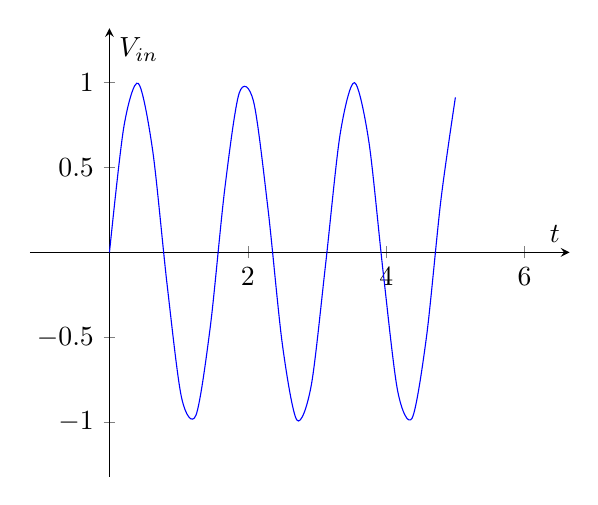
\begin{tikzpicture}
    \begin{axis}[
        domain=0:5,
        axis lines = middle,
        xmin = -0.5,
        xmax = 6,
        ymin = -1.1,
        ymax = 1.1,
        xlabel = $t$,
        ylabel = $V_{in}$,
        enlargelimits = true,
    ]
        \addplot[smooth,mark=none,color=blue] {sin(4*deg(x))};
    \end{axis}
\end{tikzpicture}
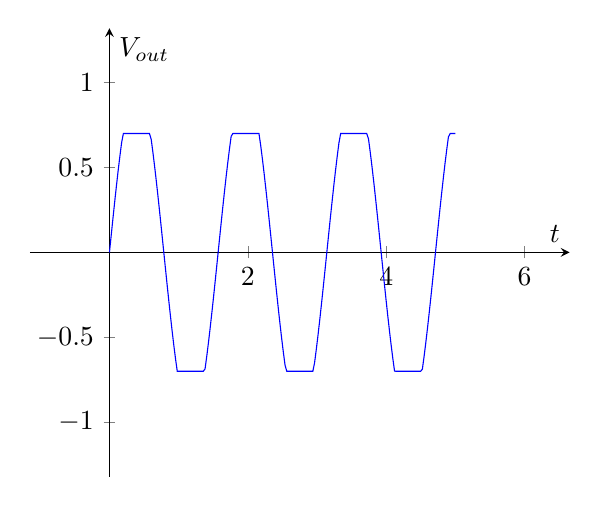
\begin{tikzpicture}
    \begin{axis}[
        domain=0:5,
        axis lines = middle,
        xmin = -0.5,
        xmax = 6,
        ymin = -1.1,
        ymax = 1.1,
        xlabel = $t$,
        ylabel = $V_{out}$,
        enlargelimits = true,
        y filter/.expression={y > 0.7 ? 0.7 : (y < -0.7 ? -0.7 : y)},
    ]
        \addplot[samples=200,mark=none,color=blue] {sin(4*deg(x))};
    \end{axis}
\end{tikzpicture}

  \caption{Impact of the diode limiter on the input sinusoidal voltage. Values that exceed the \SIrange{-0.7}{0.7}{V} range are clamped and the signal is distorted.}
  \label{fig:diode_limiter_signal}
\end{figure}


%%%%%%%%%%%%%%%%%%%%%%%%%%%%%%%%%%%%%%%%%%%%%%%%%%%%%%%%%%%%%%%%%%%%%%%%%%%%%%%%%%%%%%%
\subsection{First-Order Diode Clipper}
%%%%%%%%%%%%%%%%%%%%%%%%%%%%%%%%%%%%%%%%%%%%%%%%%%%%%%%%%%%%%%%%%%%%%%%%%%%%%%%%%%%%%%%
Combining the RC lowpass filter (\Figure{fig:rc_lowpass}) and the diode limiter (\Figure{fig:diode_limiter}) yields the first-order diode clipper (\Figure{fig:diode_clipper_circuit}). It is called "first-order" because only a single capacitor is used \cite{Parker2019}. If the input voltage is within the limiter's operational range, the circuit acts as a lowpass filter. If the voltage exceeds this range, it is clipped at the output and distortion is introduced.

The first-order diode clipper can be described by a nonlinear \ac{ODE} \cite{Yeh2007}
\begin{equation}
  \frac{\mathrm{d} V_\text{out}}{\mathrm{d}t} = \frac{V_\text{in} - V_\text{out}}{RC} - 2 \frac{I_\text{s}}{C} \sinh \left(\frac{V_\text{out}}{V_\text{t}}\right),
  \label{eq:diode_clipper_equation}
\end{equation}
where $V_\text{in}$ is the input voltage, $V_\text{out}$ is the output voltage, $t$ denotes time, $R$ is the serial resistance, $C$ is the parallel capacity, $I_\text{s}$ is the reverse saturation current, and $V_\text{t}$ is the thermal voltage. The last two are parameters of the diodes that can be measured \cite{Yeh2007}.

The parameter values of discrete elements used in the experiments were taken from \cite{Yeh2008}. They are summarized in \Table{tab:diode_clipper_element_parameters}.

\begin{table}
  \centering
  \caption{Parameter values of the discrete elements used in the diode clipper circuit. Source: \cite{Yeh2008}.}
  \begin{tabular}{c|c}
    \toprule
    \textbf{Parameter} & \textbf{Value} \\
    \midrule
    $R$ & \SI{2.2}{k\ohm} \\
    $C$ & \SI{10}{nF} \\
    $I_\text{s}$ & \SI{2.52}{nA} \\
    $V_\text{t}$ & \SI{45.3}{mV} \\
    \hline
  \end{tabular}
  \label{tab:diode_clipper_element_parameters}
\end{table}

$V_\text{in}$ is typically on the order of volts.

%%%%%%%%%%%%%%%%%%%%%%%%%%%%%%%%%%%%%%%%%%%%%%%%%%%%%%%%%%%%%%%%%%%%%%%%%%%%%%%%%%%%%%%
\subsection{Relation to Other Work}
%%%%%%%%%%%%%%%%%%%%%%%%%%%%%%%%%%%%%%%%%%%%%%%%%%%%%%%%%%%%%%%%%%%%%%%%%%%%%%%%%%%%%%%

The first-order diode clipper is a system particularly interesting in the context of ODENet, because it is governed by a known \ac{ODE} \cite{Yeh2007,Yeh2008}. Additionally, it was already modeled using a \ac{ResNet}-like architecture in \cite{Parker2019}. Thus, learning to imitate the diode clipper allowed the validation of ODENet and comparison to 
\begin{itemize}
    \item an \ac{LSTM}-based architecture from \cite{Wrightetal2020},
    \item a \ac{ResNet}-like architecture from \cite{Parker2019}, and
    \item a numerical solution using the \ac{ODE} from \cite{Yeh2007,Yeh2008}.
\end{itemize}

  \caption{Diode clipper circuit.}
  \label{fig:diode_clipper_circuit}
\end{figure}

The first-order diode clipper is a circuit frequently used to achieve signal distortion, e.g., in guitar amplifiers. Its schematic is shown in \Figure{fig:diode_clipper_circuit}. It can be regarded as consisting of two parts: an RC lowpass filter and a diode limiter.

Voltages and currents in this section are dependent on time, i.e., $V = V(t), I= I(t)$. For readability, this dependence is not stated explicitly in the equations.

%%%%%%%%%%%%%%%%%%%%%%%%%%%%%%%%%%%%%%%%%%%%%%%%%%%%%%%%%%%%%%%%%%%%%%%%%%%%%%%%%%%%%%%
\subsection{RC Lowpass Filter}
%%%%%%%%%%%%%%%%%%%%%%%%%%%%%%%%%%%%%%%%%%%%%%%%%%%%%%%%%%%%%%%%%%%%%%%%%%%%%%%%%%%%%%%

\begin{figure}
  \centering
  \begin{tikzpicture}
%--------start graphics code --------
% \draw[step=0.5,very thin, black!20] (-1,-0.5) grid (6,2.5);
\path (0,0) coordinate (ref_gnd);
\draw
  (ref_gnd)++(0,2) node[ocirc] {}
  node[xshift=-2mm,yshift=4mm] {$V_{in}$}
  to [R=\(R\)] ++(2,0) node[circ] {}
  to ++(1,0)  node[ocirc] {}
  node[yshift=4mm] {$V_{out}$}
  ++(-1,0)
  to [C=\(C\)] ++(0,-2)
  node[ground] {};
%--------end graphics code ----------
\end{tikzpicture}

  \caption{RC lowpass filter.}
  \label{fig:rc_lowpass}
\end{figure}

The first part of the diode clipper circuit is an RC lowpass filter. An RC lowpass filter is shown in \Figure{fig:rc_lowpass}. Given that the input voltage $V_\text{in}$ is a sine wave at frequency $f$, the input-output voltage relation is governed by the following equation
\begin{equation}
  V_\text{out} = \frac{X_C}{\sqrt{R^2 + X_C^2}} V_\text{in},
  \label{eq:rc_circuit}
\end{equation}
where $V_\text{out}$ is the output voltage, $X_C=\frac{1}{2\pi f C}$ is the capacitive reactance of the capacitor in the circuit, $C$ is its capacitance, and $R$ is the resistor's resistance.

The capacitor impedes low frequencies more; the lower the frequency, the higher the capacitive reactance. More capacitive reactance means larger voltage drop on the capacitor. Thus, assuming a constant magnitude across all frequencies of the input voltage, the output voltage is higher for low frequencies. Therefore, the circuit behaves like a lowpass filter.

Considering an arbitrary input waveform, we may derive a differential equation that describes the circuit \cite{Horowitz2015}. The current $I$ through the capacitor is proportional to the rate of change of the voltage across it

\begin{equation}
  I = C \frac{\mathrm{d}V_\text{out}}{\mathrm{d} t}.
  \label{eq:current_through_capacitor}
\end{equation}

The current flowing through the resistor can be calculated using the Ohm's law as a ratio of the voltage drop across the resistor to its resistance

\begin{equation}
  I = \frac{V_\text{in} - V_\text{out}}{R}.
  \label{eq:current_through_resistor}
\end{equation}

Because the same current flows through the resistor and the capacitor we can equate the right-hand sides of \Equation{eq:current_through_capacitor} and \Equation{eq:current_through_resistor}. After dividing by $C$, we obtain the final form of the \ac{ODE} describing the RC circuit

\begin{equation}
  \frac{\mathrm{d}V_\text{out}}{\mathrm{d} t} = \frac{V_\text{in} - V_\text{out}}{RC}.
\end{equation}



%%%%%%%%%%%%%%%%%%%%%%%%%%%%%%%%%%%%%%%%%%%%%%%%%%%%%%%%%%%%%%%%%%%%%%%%%%%%%%%%%%%%%%%
\subsection{Diode Limiter}
%%%%%%%%%%%%%%%%%%%%%%%%%%%%%%%%%%%%%%%%%%%%%%%%%%%%%%%%%%%%%%%%%%%%%%%%%%%%%%%%%%%%%%%
\begin{figure}
  \centering
  \begin{tikzpicture}
%--------start graphics code --------
% \draw[step=0.5,very thin, black!20] (-1,-0.5) grid (6,2.5);
\path (0,0) coordinate (ref_gnd);
\draw
  (ref_gnd)++(0,2) node[ocirc] {}
  node[xshift=-2mm,yshift=4mm] {$V_{in}$}
  to [R=\(R\)] ++(2,0) node[circ] {}
  to ++(2,0)  node[circ] {}
  to ++(1,0)  node[ocirc] {} {}
  node[yshift=4mm] {$V_{out}$}
  ++(-1,0)
  to [D] ++(0,-2)
  to ++(-1,0)
  node[ground] {}
  to ++(-1,0)
  to [D] ++(0,2);
%--------end graphics code ----------
\end{tikzpicture}

  \caption{Diode limiter circuit.}
  \label{fig:diode_limiter}
\end{figure}

The second part of the diode clipper is the diode limiter also called a \emph{diode clamp} \cite{Malvino2016}. Its circuit is shown in \Figure{fig:diode_limiter}. It consists of two inversely polarized diodes and a resistor. This circuit could be further divided into a \emph{positive clipper} (by removing the diode on the left) and a \emph{negative clipper} (by removing the diode on the right). These names refer to which part of the input \ac{AC} signal (the positive or the negative) is removed at the output.

If the diodes were ideal, i.e., they would behave as an open for voltages across smaller than 0 and as a short for voltages across larger than 0, $V_\text{out}$ would always be 0. However, to a second approximation, the diodes cause a voltage drop of \SI{0.7}{V} when conducting. Thus, the voltage cannot exceed the \SIrange{-0.7}{0.7}{V} range, being clamped when attempting to do so. The positive clipper guards the upper limit and the negative clipper guards the lower limit. The effect of passing an \ac{AC} signal through the diode limiter is shown in \Figure{fig:diode_limiter_signal}.

\cite{Yeh2007} contains a small-signal interpretation of the diode limiter circuit.

\begin{figure}
  \centering
  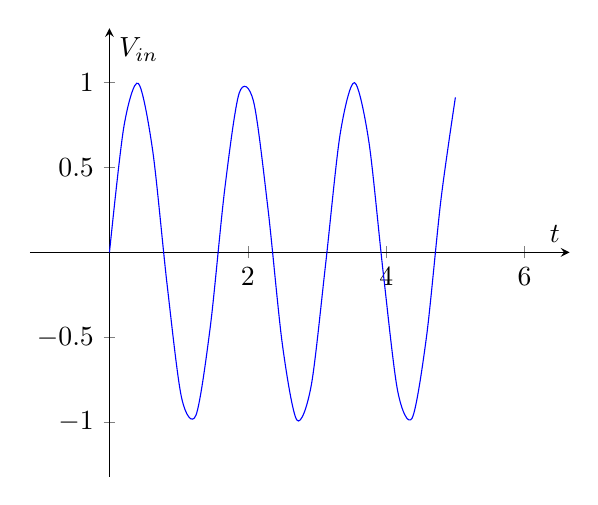
\begin{tikzpicture}
    \begin{axis}[
        domain=0:5,
        axis lines = middle,
        xmin = -0.5,
        xmax = 6,
        ymin = -1.1,
        ymax = 1.1,
        xlabel = $t$,
        ylabel = $V_{in}$,
        enlargelimits = true,
    ]
        \addplot[smooth,mark=none,color=blue] {sin(4*deg(x))};
    \end{axis}
\end{tikzpicture}
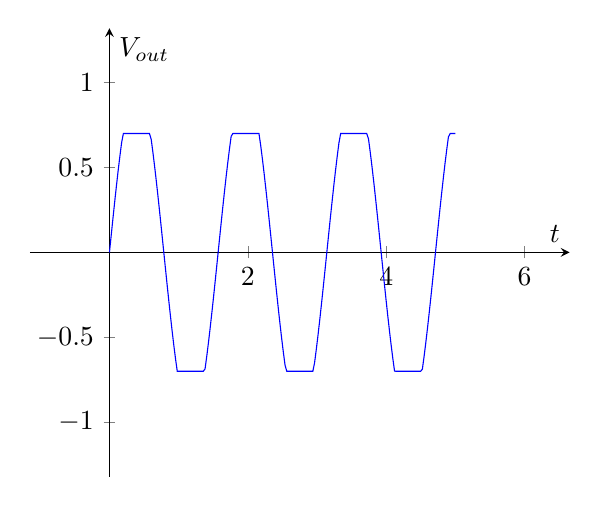
\begin{tikzpicture}
    \begin{axis}[
        domain=0:5,
        axis lines = middle,
        xmin = -0.5,
        xmax = 6,
        ymin = -1.1,
        ymax = 1.1,
        xlabel = $t$,
        ylabel = $V_{out}$,
        enlargelimits = true,
        y filter/.expression={y > 0.7 ? 0.7 : (y < -0.7 ? -0.7 : y)},
    ]
        \addplot[samples=200,mark=none,color=blue] {sin(4*deg(x))};
    \end{axis}
\end{tikzpicture}

  \caption{Impact of the diode limiter on the input sinusoidal voltage. Values that exceed the \SIrange{-0.7}{0.7}{V} range are clamped and the signal is distorted.}
  \label{fig:diode_limiter_signal}
\end{figure}


%%%%%%%%%%%%%%%%%%%%%%%%%%%%%%%%%%%%%%%%%%%%%%%%%%%%%%%%%%%%%%%%%%%%%%%%%%%%%%%%%%%%%%%
\subsection{First-Order Diode Clipper}
%%%%%%%%%%%%%%%%%%%%%%%%%%%%%%%%%%%%%%%%%%%%%%%%%%%%%%%%%%%%%%%%%%%%%%%%%%%%%%%%%%%%%%%
Combining the RC lowpass filter (\Figure{fig:rc_lowpass}) and the diode limiter (\Figure{fig:diode_limiter}) yields the first-order diode clipper (\Figure{fig:diode_clipper_circuit}). It is called "first-order" because only a single capacitor is used \cite{Parker2019}. If the input voltage is within the limiter's operational range, the circuit acts as a lowpass filter. If the voltage exceeds this range, it is clipped at the output and distortion is introduced.

The first-order diode clipper can be described by a nonlinear \ac{ODE} \cite{Yeh2007}
\begin{equation}
  \frac{\mathrm{d} V_\text{out}}{\mathrm{d}t} = \frac{V_\text{in} - V_\text{out}}{RC} - 2 \frac{I_\text{s}}{C} \sinh \left(\frac{V_\text{out}}{V_\text{t}}\right),
  \label{eq:diode_clipper_equation}
\end{equation}
where $V_\text{in}$ is the input voltage, $V_\text{out}$ is the output voltage, $t$ denotes time, $R$ is the serial resistance, $C$ is the parallel capacity, $I_\text{s}$ is the reverse saturation current, and $V_\text{t}$ is the thermal voltage. The last two are parameters of the diodes that can be measured \cite{Yeh2007}.

The parameter values of discrete elements used in the experiments were taken from \cite{Yeh2008}. They are summarized in \Table{tab:diode_clipper_element_parameters}.

\begin{table}
  \centering
  \caption{Parameter values of the discrete elements used in the diode clipper circuit. Source: \cite{Yeh2008}.}
  \begin{tabular}{c|c}
    \toprule
    \textbf{Parameter} & \textbf{Value} \\
    \midrule
    $R$ & \SI{2.2}{k\ohm} \\
    $C$ & \SI{10}{nF} \\
    $I_\text{s}$ & \SI{2.52}{nA} \\
    $V_\text{t}$ & \SI{45.3}{mV} \\
    \hline
  \end{tabular}
  \label{tab:diode_clipper_element_parameters}
\end{table}

$V_\text{in}$ is typically on the order of volts.

%%%%%%%%%%%%%%%%%%%%%%%%%%%%%%%%%%%%%%%%%%%%%%%%%%%%%%%%%%%%%%%%%%%%%%%%%%%%%%%%%%%%%%%
\subsection{Relation to Other Work}
%%%%%%%%%%%%%%%%%%%%%%%%%%%%%%%%%%%%%%%%%%%%%%%%%%%%%%%%%%%%%%%%%%%%%%%%%%%%%%%%%%%%%%%

The first-order diode clipper is a system particularly interesting in the context of ODENet, because it is governed by a known \ac{ODE} \cite{Yeh2007,Yeh2008}. Additionally, it was already modeled using a \ac{ResNet}-like architecture in \cite{Parker2019}. Thus, learning to imitate the diode clipper allowed the validation of ODENet and comparison to 
\begin{itemize}
    \item an \ac{LSTM}-based architecture from \cite{Wrightetal2020},
    \item a \ac{ResNet}-like architecture from \cite{Parker2019}, and
    \item a numerical solution using the \ac{ODE} from \cite{Yeh2007,Yeh2008}.
\end{itemize}

\section{Phaser Modeling}

This section presents the results of phaser modeling in a manner analogous to the diode clipper results presented in the previous section.

%%%%%%%%%%%%%%%%%%%%%%%%%%%%%%%%%%%%%%%%%%%%%%%%%%%%%%%%%%%%%%%%%%%%%%%%%%%%%%%%%%%%%%%
\subsection{Training Data}
\label{sec:phaser_training_data}
%%%%%%%%%%%%%%%%%%%%%%%%%%%%%%%%%%%%%%%%%%%%%%%%%%%%%%%%%%%%%%%%%%%%%%%%%%%%%%%%%%%%%%%

The training data consisted solely of guitar recordings taken from the Fraunhofer IDMT database \cite{Kehling2014}. Some of the recordings were additionally distorted using a software distortion plug-in. The purpose of applying additional distortion was to make the effect of phaser application more audible thanks to the harmonic-rich spectrum of distorted signals. The underlying assumption was that the network would learn better from these more pronounced parts. Additionally, they should make the evaluation task easier during listening tests. 

The acoustic, electric, and distorted guitar recordings were evenly split among the training, validation, and test sets. The training set was 5 minutes 44 seconds long, the validation set was 1 minute 6 seconds long, and the test set was 1 minute 49 seconds long. Audio data was single-channel at \SI{44100}{Hz} sampling rate.

The dataset was synthesized using the digital model of a phaser from \cite{Kiiski2016} with the feedback turned off. The purpose of using synthesized data instead of recorded data was to provide a ground truth LFO signal. This was the approach taken for the initial validation in \cite{Wright2020}. If a recording had been used, we would have needed to estimate the LFO signal, which could obscure the analysis. The LFO signal used for the synthesis was a rectified sine at \SI{17}{Hz}. Again, since the purpose of the training was to validate if the ODENet architecture could be applied to phaser modeling, only one type and rate of the LFO signal were used. If the answer was positive, more LFO waveforms and frequencies would be used (probably involving some not seen during training at test time). 

%%%%%%%%%%%%%%%%%%%%%%%%%%%%%%%%%%%%%%%%%%%%%%%%%%%%%%%%%%%%%%%%%%%%%%%%%%%%%%%%%%%%%%%
\subsection{Training}
\label{sec:phaser_training}
%%%%%%%%%%%%%%%%%%%%%%%%%%%%%%%%%%%%%%%%%%%%%%%%%%%%%%%%%%%%%%%%%%%%%%%%%%%%%%%%%%%%%%%
The training procedure was identical to the one for the diode clipper as described in \Section{sec:diode_clipper_training}. The only difference was that the validation loss was computed every 10 epochs instead of every epoch. 

The loss functions used for the training and the validation were the average distance measures in the time-frequency domain as described in \Section{sec:loss_functions}. Different distance measures allowed to observe different characteristics of ODENet. All models were trained and tested on data at \SI{44100}{Hz} sampling rate.

% It was chosen because of superior validation performance at high frequencies when used to train the baseline (\ac{LSTM}) in comparison to $L_1$ and $L_2$ distances in the \ac{STFT} domain as well as the \ac{ESR}.

%%%%%%%%%%%%%%%%%%%%%%%%%%%%%%%%%%%%%%%%%%%%%%%%%%%%%%%%%%%%%%%%%%%%%%%%%%%%%%%%%%%%%%%
\subsection{Compared Models}
\label{sec:phaser_models}
%%%%%%%%%%%%%%%%%%%%%%%%%%%%%%%%%%%%%%%%%%%%%%%%%%%%%%%%%%%%%%%%%%%%%%%%%%%%%%%%%%%%%%%

In the case of the phaser models, only the ODENet framework was compared to the baseline: an \ac{LSTM} from \cite{Wright2020} with 16 memory cells (\ac{LSTM}16). For the derivative network a sufficiently large \ac{MLP} was chosen. Its dimensionality was $M + 2 \times 30 \times 60 \times 60\times 60 \times 30\times M$, where $M$ was the manually set size of the state vector. The nonlinearity used was \ac{SELU}. To prevent divergence, we added a weight decay term to the loss function as a regularizer.

\begin{table}[]
    \caption{Compared network architectures for phaser modeling}
    \centering
    \begin{tabular}{@{}l|c c @{}}
\toprule
Model & LSTM16 & ODENet \\ \midrule % state_size = 36, hidden_size = 30
Number of   parameters & 1297 & \makecell{11161 (state size 1)\\12198 (state size 18)\\13296 (state size 36)} \\
Weight decay & 1e-7 & 1e-7             \\
Learning rate & 0.001 & 0.0005            \\
Learning rate schedule & none & one cycle LR 0.003      \\
Epochs in training & 1000 & 1200            \\
Hours in training & 3.5 & 22.5           \\
Teacher forcing & never & always       \\ 
Minibatch size & 64 &   256  \\ \bottomrule
\end{tabular}%

    \label{tab:phaser_models_data}
\end{table}

%%%%%%%%%%%%%%%%%%%%%%%%%%%%%%%%%%%%%%%%%%%%%%%%%%%%%%%%%%%%%%%%%%%%%%%%%%%%%%%%%%%%%%%
\subsection{Results and Discussion}
\label{sec:phaser_results}
%%%%%%%%%%%%%%%%%%%%%%%%%%%%%%%%%%%%%%%%%%%%%%%%%%%%%%%%%%%%%%%%%%%%%%%%%%%%%%%%%%%%%%%

The goal of phaser modeling was not only to compare ODENet to the approach taken in \cite{Wright2020} but also to verify the assumption on the state augmentation. The assumption was that the derivative network can use the unobserved entries in the state vector to store information helpful in obtaining more accurate results.

%%%%%%%%%%%%%%%%%%%%%%%%%%%%%%%%%%%%%%%%%%%%%%%%%%%%%%%%%%%%%%%%%%%%%%%%%%%%%%%%%%%%%%%
\subsubsection{The Impact of State Augmentation}
%%%%%%%%%%%%%%%%%%%%%%%%%%%%%%%%%%%%%%%%%%%%%%%%%%%%%%%%%%%%%%%%%%%%%%%%%%%%%%%%%%%%%%%
The effect of augmenting the state vector from 1 to 18 entries when training with the average $L_1$ distance in the \ac{STFT} domain can be seen in \Figure{fig:state_augmentation}. Although no target was provided for the 17 latent entries, the network used them to store meaningful information for each time point. The observed improvement is over two-fold. Therefore, it may be beneficial to augment the state, even if the training signal is not provided for all of its entries. However, the improvement was not observed when $L_2$ or $LSD_\text{RMS}$ distances were used.

\begin{figure}
    \centering
    \begin{tikzpicture}
    \begin{axis}[
        no markers,
        every axis plot/.append style={ultra thick},
        xmin = 0,
        xmax = 1200,
        ymin = 0,
        grid,
        xlabel = Epoch,
        ylabel = Validation Loss,
    ]
        \addplot[smooth,mark=none,color=red] table [x=Step, y=Value, col sep=comma] {figures/tikz/state_augmentation/State_size_1_L1_STFT-tag-Loss_validation.csv};
        \addplot[smooth,mark=none,color=green] table [x=Step, y=Value, col sep=comma] {figures/tikz/state_augmentation/State_size_36_L1_STFT_DerivativeMLP2-tag-Loss_validation.csv};
        \legend{state size 1, state size 18};
    \end{axis}
\end{tikzpicture}

    \caption{Average $L_1$ loss of ODENet in the \ac{STFT} domain on the validation set with and without state augmentation.}
    \label{fig:state_augmentation}
\end{figure}

%%%%%%%%%%%%%%%%%%%%%%%%%%%%%%%%%%%%%%%%%%%%%%%%%%%%%%%%%%%%%%%%%%%%%%%%%%%%%%%%%%%%%%%
\subsubsection{Comparison to the Baseline}
%%%%%%%%%%%%%%%%%%%%%%%%%%%%%%%%%%%%%%%%%%%%%%%%%%%%%%%%%%%%%%%%%%%%%%%%%%%%%%%%%%%%%%%

Test results of phaser modeling are shown in \Table{tab:phaser_results}, where $LSD_\text{RMS}$ was defined in \Equation{eq:log_spectral_distance}, \ac{segSNR} was defined in \Equation{eq:seg_snr}, and \ac{PEAQ} was explained in \Section{subsec:va_evaluation}. The $LSD_\text{RMS}$  loss was chosen for the final training and comparison, because during a visual inspection of the magnitude \ac{STFT} it resulted in the best match of phaser notches in the output signal of the baseline model. It was assumed that it would enable effective learning for ODENet as well.

\begin{table}[]
    \caption{Test results of the phaser models.}
    \centering
    \newcommand{\modelNameCellWidth}{1.8cm}
    \begin{tabular}{@{} l | c c @{}}
        \toprule
        Model & LSTM16 & ODENet \\ \midrule
        Loss    & \textbf{4.7\%} & TBF \\
        segSNR  & \textbf{8.5} & TBF  \\
        ODG     & \textbf{-0.27} & TBF \\ \bottomrule
    \end{tabular}%
    
    \label{tab:phaser_results}
\end{table}

In terms of numerical measures, \ac{LSTM}16 significantly outperformed ODENet. The validation curves of both models can be seen in \Figure{fig:phaser_lstm_vs_fe}. \ac{LSTM}16 has smaller dynamics of learning, which could point to the fact that it is more suited for modeling the phaser.

\begin{figure}
    \centering
    \begin{tikzpicture}
    \begin{axis}[
        no markers,
        every axis plot/.append style={ultra thick},
        xmin = 0,
        xmax = 1200,
        ymin = 0,
        grid,
        xlabel = Epoch,
        ylabel = Validation Loss,
    ]
        \addplot[smooth,mark=none,color=blue] table [x=Step, y=Value, col sep=comma] {figures/tikz/phaser_lstm_vs_fe/LSTM_L1_STFT.csv};
        \addplot[smooth,mark=none,color=green] table [x=Step, y=Value, col sep=comma] {figures/tikz/phaser_lstm_vs_fe/FE_L1_STFT.csv};
        \legend{LSTM16, ODENet};
    \end{axis}
\end{tikzpicture}

    \caption{Average $LSD_\text{RMS}$ of the compared models on the validation set.}
    \label{fig:phaser_lstm_vs_fe}
\end{figure}

The results in the \ac{STFT} domain can be seen in \Figure{fig:phaser_test_spectrograms}. The notches learned by \ac{LSTM}16 closely match those of the target. The notches learned by ODENet are almost invisible (although they are present at closer inspection). It must also be stated that ODENet always diverged during test, what can be seen in the range of values in the colorbar.

\newcommand{\scaleboxsizee}{0.8}
\begin{figure}
    \centering
    \begin{subfigure}{0.7\textwidth}
        \centering
        \scalebox{0.81}{% This file was created by tikzplotlib v0.9.6.
\begin{tikzpicture}

\begin{axis}[
colorbar,
colorbar style={ytick={-40,-20,-7.105427357601e-15,20},yticklabels={\(\displaystyle -40\),\(\displaystyle -20\),\(\displaystyle 0\),\(\displaystyle 20\)},ylabel={}},
colormap/viridis,
point meta max=22.9006375273498,
point meta min=-54.103633370184,
tick align=outside,
tick pos=left,
x grid style={white!69.0196078431373!black},
xlabel={Time [s]},
xmin=0, xmax=14.9072108843537,
xtick style={color=black},
xtick={0,5,10,15},
xticklabels={\(\displaystyle 0\),\(\displaystyle 5\),\(\displaystyle 10\),\(\displaystyle 15\)},
y grid style={white!69.0196078431373!black},
ylabel={Frequency [kHz]},
ymin=0, ymax=22,
ytick style={color=black},
ytick={0,5,10,15,20,25},
yticklabels={\(\displaystyle 0\),\(\displaystyle 5\),\(\displaystyle 10\),\(\displaystyle 15\),\(\displaystyle 20\),\(\displaystyle 25\)}
]
\addplot graphics [includegraphics cmd=\pgfimage,xmin=0, xmax=14.9072108843537, ymin=0, ymax=22] {figures/tikz/phaser_test_spectrograms/FameSweetToneOffNoFb-test-target_stft-000.png};
\end{axis}

\end{tikzpicture}
}
    \end{subfigure}
    \begin{subfigure}{0.7\textwidth}
        \centering
        \scalebox{\scaleboxsizee}{% This file was created by tikzplotlib v0.9.6.
\begin{tikzpicture}

\begin{axis}[
colorbar,
colorbar style={ytick={-40,-20,0,20},yticklabels={\(\displaystyle -40\),\(\displaystyle -20\),\(\displaystyle 0\),\(\displaystyle 20\)},ylabel={Magnitude [dB]}},
colormap/viridis,
point meta max=21.1321993583666,
point meta min=-55.5277115981883,
tick align=outside,
tick pos=left,
x grid style={white!69.0196078431373!black},
xlabel={Time [s]},
xmin=0, xmax=14.9072108843537,
xtick style={color=black},
xtick={0,5,10,15},
xticklabels={\(\displaystyle 0\),\(\displaystyle 5\),\(\displaystyle 10\),\(\displaystyle 15\)},
y grid style={white!69.0196078431373!black},
ylabel={Frequency [kHz]},
ymin=0, ymax=22,
ytick style={color=black},
ytick={0,5,10,15,20,25},
yticklabels={\(\displaystyle 0\),\(\displaystyle 5\),\(\displaystyle 10\),\(\displaystyle 15\),\(\displaystyle 20\),\(\displaystyle 25\)}
]
\addplot graphics [includegraphics cmd=\pgfimage,xmin=0, xmax=14.9072108843537, ymin=0, ymax=22] {figures/tikz/phaser_test_spectrograms/LSTM16_log_spectral_distance_stft-000.png};
\end{axis}

\end{tikzpicture}
}
    \end{subfigure}
    \begin{subfigure}{0.7\textwidth}
        \centering
        \scalebox{\scaleboxsizee}{% This file was created by tikzplotlib v0.9.6.
\begin{tikzpicture}

\begin{axis}[
colorbar,
colorbar style={ytick={-60,-40,-20,0,20,40},yticklabels={\(\displaystyle -60\),\(\displaystyle -40\),\(\displaystyle -20\),\(\displaystyle 0\),\(\displaystyle 20\),\(\displaystyle 40\)},ylabel={Magnitude [dB]}},
colormap/viridis,
point meta max=49.2661401752569,
point meta min=-61.6565473918622,
tick align=outside,
tick pos=left,
x grid style={white!69.0196078431373!black},
xlabel={Time [s]},
xmin=0, xmax=14.9072108843537,
xtick style={color=black},
xtick={0,5,10,15},
xticklabels={\(\displaystyle 0\),\(\displaystyle 5\),\(\displaystyle 10\),\(\displaystyle 15\)},
y grid style={white!69.0196078431373!black},
ylabel={Frequency [kHz]},
ymin=0, ymax=22,
ytick style={color=black},
ytick={0,5,10,15,20,25},
yticklabels={\(\displaystyle 0\),\(\displaystyle 5\),\(\displaystyle 10\),\(\displaystyle 15\),\(\displaystyle 20\),\(\displaystyle 25\)}
]
\addplot graphics [includegraphics cmd=\pgfimage,xmin=0, xmax=14.9072108843537, ymin=0, ymax=22] {figures/tikz/phaser_test_spectrograms/FE_log_spectral_distance_stft-001.png};
\end{axis}

\end{tikzpicture}
}
    \end{subfigure}
    \caption{A fragment of the magnitude \ac{STFT} of the models' test output. (Top) Target. (Middle) \ac{LSTM}16. (Bottom) ODENet (state size 36).}
    \label{fig:phaser_test_spectrograms}
\end{figure}

In casual listening, \ac{LSTM}16 sounds indistinguishable from the target. On the contrary, the output of ODENet does not sound as processed with phaser at all. The gentle notches that can be seen under a close inspection of ODENet output spectrograms are not audible.

Ultimately, we were not able to achieve a better performance of ODENet on the phaser dataset. This suggests that ODENet may not be able to learn the instantaneous derivative of the phaser system.

